\chapter{Introduction}


In questo capitolo ci occuperemo di analizzare e comprendere delle vulnerabilità
del protocollo DDS standard OMG (Object Management Group). In particolare
verrà analizzato il vettore d'attacco, il protocollo utilizzato, il bersaglio
dell'attacco e infine verrà proposta una soluzione applicabile per
mitigare possibili attacchi non autorizzati. Nel prossimo capitolo grazie all'aiuto
del software --inserire software-- riusciremo a capire come queste vulnerabilità
possono essere ricreate in un ambiente simulato.
Queste vulnerabilità di base hanno una base una base di appoggio solida per 
l'attaccante, in molti casi un dispositivo ha già a disposizione il controllo
di un partecipante all'interno della rete o ha la possibilità di modificare
dei file di configurazione all'interno della rete DDS.

Di seguito la versione del DDS con lo standard OMG utilizzata in tutti i casi è
la 1.4




\section{Attacchi DDoS}
Questi attacchi consistono nel sovraccaricare uno o più dispositivi collegati alla 
rete DDS in modo tale da renderli non responsive. Infatti molti sono di tipo 
I O T -- e la potenza di calcolo nella maggior parte dei casi è ridotta.
Per di più in molti casi vengono utilizzati dispositivi
che non possono permettersi --delay-- nell'analisi di certi dati, specialmente in
ambiti RealTime in cui bisogna avere delle risposte rapide, come ad esempio
nel campo della medicina e nel campo militare.


\subsection{DDoS blocco ricezione da parte del datareader Foglio 2}

%\subsubsection{Prologo}
Citazioni da foglio 2 a gogo
Il vettore di attacco si trova nel protocollo RTPS che
si occupa di scambiare pacchetti tra i DataReader (coloro che si iscrivono ai vari
ai vari topic) e i DataWriter (di solito sono sensori che inviano dati).
Questo protocollo utilizza il messaggio HEARTBEAT che viene mandato da un DataWriter
a un DataReader per specificare il sequence number del DataWriter.
Il sequence number serve al DataReader per sincronizzarsi con il DataWriter 
durante la ricezione dei pacchetto.
Infatti il DataReader quando riceve il sequence number all'interno di un HEARTBEAT
può identificare se ci sono o no dei pacchetti mancanti e in caso segnalarli al
DataWriter.


Un DataWriter inoltre può richiedere un messaggio ACKNACK da un DataReader se
nell'HEARTBEAT inviato in precedenza dal DataWriter il parametro FINAL è attivo.
Il messaggio ACKNACK consente di far rimanere sempre sincronizzato il DataReader al 
DataWriter che non potrà spedire nuovi pacchetti HEARTBEAT fino a quando non ha 
ricevuto la conferma di ricezione con un messaggio ACKNACK.
I controlli del sequence number all'interno dell'HEARTBEAT 
non sono sufficienti per coprire la rete da questo tipo di attacco:
\begin{itemize}
    \item un controllo viene effettuato per verificare che non ci siano 
    valori negativi
    \item un altro controllo serve a determinare se l'ultimo sequence number 
    appena ricevuto non ha un valore più alto di quello ricevuto in precedenza
\end{itemize}
\subsubsection{Dettagli attacco AFTER}

Per sfruttare questa vulnerabilità l'attaccante deve utilizzare qualche 
strumento per sniffare la comunicazione tra il DataReader e il DataWriter,
intercettando i
messaggi HEARTBEAT. Dopo aver catturato un pacchetto di tipo HEARTBEAT e modificato 
il suo sequence number assegnandogli un valore molto alto, 
l'attaccante lo invia al DataReader.
Una volta ricevuto il pacchetto il DataReader si metterà in attesa di un HEARTBEAT 
con un
sequence number superiore a quello appena ricevuto. Di conseguenza il DataReader
non elaborerà più i messaggi legittimi mandati dal DataWriter,
data che hanno sequence numember più piccoli, bloccando così la sua
esecuzione indefinitamente. Solo un messaggio HEARTBEAT con un sequence number
maggiore a quello del DataReader farà ripristinare la sua esecuzione.


\subsubsection{Conclusioni AFTER}
Di solito questo tipo di attacco è difficile da identificare. 
Un messaggio HEARTBEAT riguarda un solo topic e quindi il resto delle
comunicazione che avvengono su topic differenti o anche sullo stesso 
topic, ma con un DataReader diverso, non subiranno cambiamenti.


\subsection{DDoS sfruttando estensione DDS security}
In questo attacco dobbiamo considerare il modulo del DDS chiamato DDS security
versione 1.1.(fonti ora da foglio 6) Questo modulo si occupa di stabilire una
connessione sicura tra i vari dispositivi della rete. Infatti verranno utilizzate
delle api da parte dei partecipanti per effettuare le varie azioni, come
ad esempio iscriversi ad un topic e pubblicare un messaggio del topic.
(foglio 3 pag 718)Per effettuare l'autenticazione un partecipante deve prima
risolvere una challenge crittografica richiesta dal sistema di autenticazione
della rete. Effettuato poi questo calcolo criptografico il risultato viene
controllato dal sistema di autenticazione, controllando che se il risultato
inviato corrisponde all'hash della challenge crittografica.


\subsubsection{Dettagli attacco AFTER foglio 3}
L'attacco DDoS si svolge proprio durante la fase di autenticazione del protocollo
DDS security 1.1, in particolare quando un nuovo dispositivo legittimo si vuole
collegare alla rete e comincia a mandare una richiesta di autenticazione
all'ente di controllo. La richiesta del partecipante poi viene intercettata
dall'attaccante che modifica i valori all'interno del pacchetto delle
challenge crittografica. Modificando ogni volta questi valori, l'attaccante
comincia a mandare tante richieste crittografiche alla sua vittima.
Il partecipante comincerà a calcolare queste challenge per effettuare
l'autenticazione investendo tutte le risorse necessarie.
Dato che molto probabilmente chi riceve questo attacco è un dispositivo IOT
che non dispone di una potenza di calcolo molto elevata e si ritroverà
occupato per tutto il tempo necessario per risolvere le challenge crittografiche
ricevute dall'attaccante, bloccando così il suo funzionamento.


\subsubsection{Conclusioni AFTER foglio 3}
Una raccomandazione per mitigare questo attacco può essere quello di cambiare delle
policy QoS in modo tale da impostare un tempo limite massimo per effettuare
l'autenticazione. Impostando un limite simile queste policy possono prevenire
che i partecipanti si ritrovino sopraffatti dalle troppe richieste di
autenticazione. Un allarme potrebbe essere anche utile per identificare possibili
tentativi DDoS di questo tipo così allertando un amministratore. (parlare di proverif)


\section{Attacchi di enumerazione e di sniffing}
Dal foglio 2
Prendere informazioni DDS senza effettuare veri e propri
attacchi di tipo attivo può essere molto utile per un attaccante che prova
a penetrare una rete DDS. In molti casi tutto quello che deve fare l'attaccante
è osservare i messaggi che vengono scambiati all'interno del network.
Successivamente quando si ottengono informazioni a sufficienza sarà più
facile per l'attaccante trovare un vettore di attacco.


\subsection{Enumeration sniff foglio 2 e foglio 5}
Prendendo in considerazione il protocollo DDSI-RTPS, possiamo notare che di
default quest'ultimo è molto "verbose", cioè scambia molte informazioni in
chiaro durante le comunicazioni tra i vari dispositivi. In particolare
il modulo discovery del protocollo RTPS che a sua volta si suddivide in
altri 2 protocolli fondamentali che sono necessari:(foglio 5 pag 123)
\begin{itemize}
    \item Simple Participant Discovery Protocol (SPDP)
    \item Simple Endpoint Discovery Protocol (SEDP)
\end{itemize}
Per questo attacco ci focalizzeremo in particolare nel SPDP che serve a
individuare la presenza dei partecipanti alla rete. In particolar modo
il funzionamento si basa su un messaggio di tipo multicast e unicast che viene
mandato a tutti i dispositivi della rete per informare chi è presente attualmente.
(foglio 5 pag 125)


\subsubsection{Dettagli attacco AFTER}
Utilizzando un qualche software in grado di "sniffare" i vari pacchetti della
rete, come un semplice script python è stato possibile analizzare il loro
contenuto. I pacchetti analizzati sono quelli di tipo multicast RTPS SPDP
All'interno di un pacchetto di questo tipo possiamo trovare: (nel foglio 2
non viene specificato bene di quale pacchetto si parla, ma guardando la documentazione
da pag 125 del foglio 5, stiamo analizzando il pacchetto SPDPdiscoveredParticipandData)
(da scrivere in corsivo) l'indirizzo ip dell'host, il prefisso GUID dell'RTPS,
la versione dell RTPS, L'ID del venditore, informazioni riguardanti la sincronizzazione
e infine il contenuto dei submessages.




\subsubsection{Conclusioni AFTER}
Di solito questi tipo di attacco sono difficili da identificare e possono essere
effettuati anche non avendo un dispositivo autenticato all'interno della rete.


\section{QoS Exploitation Attack foglio 1}


% \begin{figure}[H]
%     \centering
%     \includesvg[width=15cm,keepaspectratio]{img/Policy QoS DDS.drawio.svg}
%     \caption{Illustrazione policy QoS del DDS}\label{Mappa QoS svg}
% \end{figure}




\begin{figure}[H]
    \centering
    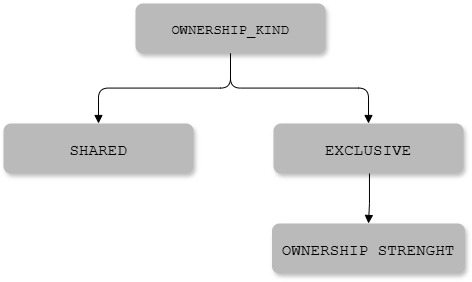
\includegraphics[width=10cm, keepaspectratio]{img/Policy QoS DDS_2.jpg}
    \caption{Illustrazione policy QoS del DDS}\label{Mappa QoS}
\end{figure}
% AFTER si potrebbe fare nei capitoli introduttivi una mappa che racchiuda
% i tipi di variabili che usano i QoS (int, double,.. etc) per i capitoli
% che spiegano meglio i concetti introduttivi


Queste tipologie di attacco sono possibili solo se certe policy QoS vengono
modificate durante l'esecuzione della rete, specialmente il parametro
OWNERSHIP-KIND che gestisce quanti DataWriter possono scrivere per un
determinato Topic. Questo parametro può essere impostato in due modi diversi:
\begin{itemize}
    \item SHARED: in questo modo più di un DataWriter possono aggiornare le
    informazioni di un topic. Inoltre un DataReader si può iscrivere a
    qualsiasi scrittore dello stesso topic.
    \item EXCLUSIVE: solo un DataWriter può aggiornare le informazioni di un
    topic. Il DataWriter che ha il permesso di scrittura per il topic è quello
    che dispone di un OWNERSHIP-strength con valore più alto.
\end{itemize}
% https://www.omgwiki.org/ddsf/doku.php?id=ddsf:public:guidebook:06_append:02_quality_of_service:ownership
% https://www.omgwiki.org/ddsf/doku.php?id=ddsf:public:guidebook:06_append:02_quality_of_service:ownership_strength


Un'altra policy QoS che può essere usata come vettore di attacco è quella
che regola il parametro LIFESPAN. Corrisponde al tempo limite massimo per la
lettura da parte di un DataReader di un dato di un topic, che viene inserito
all'interno del pacchetto inviato dal DataWriter. Per determinare se un pacchetto
di un determinato topic è scaduto viene utilizzato il timestamp di creazione
aggiungendo il LIFESPAN impostato; se questo questo "expiration time" risulta
superiore all'orario durante la ricezione del DataReader allora l'informazione
ricevuta è ancora valida. Per funzionare gli orologi del DataWriter e del DataReader
devono essere sincronizzati tra di loro.


% https://www.omgwiki.org/ddsf/doku.php?id=ddsf:public:guidebook:06_append:02_quality_of_service:lifespan




Un'altra importante policy da considerare è quella riguardo all'affidabilità
(RELIABILITY) dei dati riguardanti un topic che può essere impostata in due
modi:
\begin{itemize}
    \item RELIABLE: questa impostazione costringe il DataReader a farsi
    ritrasmettere dal DataWriter i pacchetti mancanti o ricevuti in maniera errata.
    In questo modo le informazioni del DataReader saranno sempre corrette anche
    se non sempre saranno aggiornate in tempo reale.
    \item BEST-EFFORT: l'impostazione predefinita che consente il recupero
    dei pacchetti mancanti del DataReader, quindi quest'ultimo potrebbe anche
    perdere dei pacchetti che gli sono stati inviati.
\end{itemize}




% https://www.omgwiki.org/ddsf/doku.php?id=ddsf:public:guidebook:06_append:02_quality_of_service:reliability




\subsection{Foglio 4-B Modifica maligna di ownership strength}
In una rete dove si utilizza un OWNERSHIP-kind di tipo EXCLUSIVE è possibile
utilizzare l'OWNERSHIP-strength a favore
dell'attaccante. Infatti è possibile far ricevere informazioni a un DataWriter
in maniera errata, dato che quest'ultimo non riceverà più informazioni da
una fonte affidabile.


\subsubsection{Foglio 4-B Dettagli attacco}
L'attaccante, con un DataWriter in suo possesso all'interno di una rete DDS,
può sfruttare il fatto che il topic preso di mira può essere aggiornato
solo dal DataWriter con l'OWNERSHIP-strength più alta.
Per effettuare questo attacco tutto quello che serve è sapere il topic che
si vuole modificare, le policy QoS in uso e il valore dell ownership-strength.
L'ultimo passo è quello di impostare il topic scelto nel DataWriter
dell'attaccante con OWNERSHIP-strength superiore a quella utilizzata dal
DataWriter originario che aggiorna il topic.
Ora i DataReader che sono iscritti al topic bersaglio
ricevono le informazioni dal DataWriter dell'attaccante.


\subsubsection{Foglio 4-B Conclusioni}
L'OWNERSHIP-kind di tipo EXCLUSIVE è utilizzata in contesti dove le
informazioni ricevute dal DataReader devono essere accurate dato che un singolo
scrittore (in molti casi si tratta di un sensore) può mandare nuovi aggiornamenti
del topic. Se l'attaccante, dovesse riesce a modificare i valori del topic con
questo attacco, può causare in certi casi molti danni a seconda della rete DDS,
specialmente se il DataWriter dell'attaccante riesce a mandare degli aggiornamenti
del topic senza che venga scoperto.


Una soluzione utile a risolvere questo vettore di attacco potrebbe essere l'utilizzo
dell'estensione DDS security che rende impossibile capire qual è il topic bersaglio
perchè i messaggi scambiati tra DataReader e DataWriter sono criptati.


\subsection{Foglio 4-D Modifica maligna di LIFESPAN QoS}
L'attaccante in questo attacco deve poter modificare le policy QoS riguardanti
LIFESPAN e se necessario il parametro RELIABLE.
Infatti il tempo di limite di scadenza dei pacchetti (LIFESPAN)
può essere impostato a valori molto piccoli creando problemi di comunicazione
tra un DataWriter e un DataReader. Utilizzando un'affidabilità di tipo RELIABLE
si riesce mitigare l'attaccante deve utilizzare valori più estremi per compromettere
la comunicazione. Questo test è stato dimostrando RTI Shapes Demo che implementa una
soluzione DDS di RTI corrisponde a quella dello standard OMG.


\subsubsection{Foglio 4-D Dettagli attacco}
Avendo sotto controllo questi due parametri policy, l'attaccante può modificare La
policy dei DataWriter in modo tale da avere un LIFESPAN molto piccolo. Così
facendo i pacchetti spediti dal publisher arriveranno già scaduti e non potranno
essere utilizzati dai DataReader, in certi casi il pacchetto che deve essere inviato
viene distrutto dallo stesso DataWriter all'interno della coda prima dell'invio
del pacchetto. In questo caso il test è stato effettuato impostando il valore di
LIFESPAN < 80ms dove si è visto che nessun pacchetto raggiunge il DataReader.
Se si aumenta il valore tra gli 80ms e i 100ms già si può notare che dei pacchetti
vengono letti con successo dal DataReader, mentre altri vengono eliminati prima
della lettura. Infine impostando un valore LIFESPAN >= 120ms si può notare che
la comunicazione tra publisher e subscriber avviene senza nessun problema.


Un dettaglio da aggiungere è che se su RTI Shapes veniva impostata la policy
dell'affidabilità (RELIABILITY) di tipo RELIABLE i millisecondi utilizzati
dal LIFESPAN per compromettere le comunicazioni tra DataReader e DataWriter
devono essere moltiplicati per un fattore di 0.01. Quindi ad esempio se si
ottiene un completo annullamento delle comunicazioni con un LIFESPAN < 80ms
utilizzando il la RELIABILITY di tipo BEST-EFFORT, per ottenere lo stesso
risultato con RELIABILITY di tipo RELIABLE dobbiamo impostare un
LIFESPAN < 0.8ms.


\subsubsection{Foglio 4-D Conclusioni}
Inizialmente molte reti DDS hanno impostato come parametro RELIABILITY quella
di tipo BEST-EFFORT che è l'impostazione di default. Quindi nella maggior parte
dei casi l'attaccante non si deve preoccupare di questo parametro.


Una possibile soluzione sarebbe quella di impostare qualche tipo di controllo
in modo tale da avvertire un operatore umano se molti pacchetti vengono
scartati perché arrivati con un LIFESPAN scaduto. Questo controllo potrebbe
essere anche utile, nel caso in cui il DataWriter e il DataReader si trovano
distanti fisicamente tra di loro, per verificare la qualità del collegamento.








\subsubsection{Questa è una sottosottosezione}
La teoria dell'attacco ci dice che se 

% Definizione di un colore personalizzato
\definecolor{customgray}{rgb}{0.70, 0.70, 0.70} % Grigio chiaro

% Regolazione dello spessore delle linee
\setlength{\arrayrulewidth}{1.0pt} % Spessore linee generali
% \renewcommand{\arraystretch}{1.2} % Altezza righe


\begin{table}[H]
    \centering
    \rowcolors{2}{black!5}{white}
    \resizebox{\linewidth}{!}{%
        \begin{tabular}{|c|c|c|c|c|c|}
            \hline
            \rowcolor{customgray}
            \multicolumn{1}{|>{\columncolor{customgray}}c|}{\tabularCenterstack{c}{\textbf{Tipo di}\\ \textbf{attacco}}} &
            \multicolumn{1}{>{\columncolor{customgray}}c|}{\tabularCenterstack{c}{\textbf{Vettore} \\ \textbf{attacco}}} &
            \multicolumn{1}{>{\columncolor{customgray}}c|}{\tabularCenterstack{c}{\textbf{Protoc.}/ \\ \textbf{Estens.}}} &
            \multicolumn{1}{>{\columncolor{customgray}}c|}{\tabularCenterstack{c}{\textbf{Bersaglio} \\ \textbf{nella rete}}} &
            \multicolumn{1}{>{\columncolor{customgray}}c|}{\tabularCenterstack{c}{\textbf{Software}}} &
            \multicolumn{1}{>{\columncolor{customgray}}c|}{\tabularCenterstack{c}{\textbf{Soluzione}}} \\
            \hline
            \tabularCenterstack{c}{Discovery \\ devices[2]} &
            \tabularCenterstack{c}{Verbose nature \\ of RTPS} &
            \tabularCenterstack{c}{DDSI-RTPS} &
            \tabularCenterstack{c}{Tutti i par-\\tecipanti} &
            \tabularCenterstack{c}{Sniffer \\ python} &
            \tabularCenterstack{c}{-} \\
            \specialrule{0.3pt}{0pt}{0pt} % Linea più spessa dopo l'intestazione
            \tabularCenterstack{c}{DDos[2]} &
            \tabularCenterstack{c}{Heartbeat \\ sequence number} &
            \tabularCenterstack{c}{DDSI-RTPS} &
            \tabularCenterstack{c}{DataReader} &
            \tabularCenterstack{c}{Sniffer \\ python} &
            \tabularCenterstack{c}{-} \\
            \specialrule{0.3pt}{0pt}{0pt} % Linea più spessa dopo l'intestazione
            \tabularCenterstack{c}{DDoS[3]} &
            \tabularCenterstack{c}{Authentication \\ challenge} &
            \tabularCenterstack{c}{DDS security 1.1 \\ Discovery protoc.} &
            \tabularCenterstack{c}{Tutti i par-\\tecipanti} &
            \tabularCenterstack{c}{Proverif} &
            \tabularCenterstack{c}{Scandenza richieste \\ di autenticazione} \\
            \specialrule{0.3pt}{0pt}{0pt} % Linea più spessa dopo l'intestazione
            \tabularCenterstack{c}{QoS policy[4]} &
            \tabularCenterstack{c}{ownership-strength} &
            \tabularCenterstack{c}{DDSI-RTPS} &
            \tabularCenterstack{c}{DataReader} &
            \tabularCenterstack{c}{RTI \\ shapes} &
            \tabularCenterstack{c}{DDS security} \\
            \specialrule{0.3pt}{0pt}{0pt} % Linea più spessa dopo l'intestazione
            \tabularCenterstack{c}{QoS policy[4]} &
            \tabularCenterstack{c}{LIFESPAN} &
            \tabularCenterstack{c}{DDSI-RTPS} &
            \tabularCenterstack{c}{DataReader} &
            \tabularCenterstack{c}{RTI \\ shapes} &
            \tabularCenterstack{c}{Controllo per \\ LIFESPAN scartati} \\
            \specialrule{0.3pt}{0pt}{0pt} % Linea più spessa dopo l'intestazione
            
            % Aggiungere altre linee

            \hline
        \end{tabular}
        }
        \caption{La versione DDS in tutti i casi è la 1.4}
    \end{table}




